%\documentclass[handout]{beamer}
\documentclass{beamer}
\usepackage{ru}
\usepackage{amsmath}
\usepackage{tikz}
\usepackage{epigraph}
\usepackage{xcolor}

\usetikzlibrary{arrows, calc, decorations.markings, positioning}

\usefonttheme[onlymath]{serif}

%%
%% Haal mijn eigen definities op.
\input definitions_slides.tex
%%
%%

\title{Church-Turing These}
\subtitle{Een nieuw paradijs}
\author{Pieter van Engelen}
\institute{Radboud Universiteit Nijmegen}
\date{03-06-2022@Fontys, Sittard}

\begin{document}

\begin{frame}
    \titlepage
\end{frame}

\begin{frame}
    \tableofcontents
\end{frame}

\section{De tijd}
\begin{frame}
    \begin{timeline}{1925}{1950}{2cm}{2.5cm}{7cm}{10cm}
        \entry{1928}{\small Formulering \emph{Entscheidungsproblem} in \emph{Grundzüge der theoretischen Logik}}
        \entry{1931}{\small Onvolledigheidsstellingen van Gödel}
        \entry{1932}{\small Introductie van de $\lambda$-calculus (A. Church)}
        \entry{1936}{\small Negatieve oplossing \emph{Entscheidungsproblem}}
        \entry{1937}{\small Introductie \emph{turing machine, halting problem} en negatieve oplossing \emph{Entscheidungsproblem}}
        \entry{1939}{\small \emph{Systems of logics based on ordinals} (Turing)}
        \entry{1944}{\small \emph{Introductie Turing-degree} (E. Post)}
        \entry{1945}{\small \emph{First Draft of a Report on the EDVAC} (von Neumann)}
    \end{timeline}    
\end{frame}

\begin{frame}
    \frametitle{De These}
    \begin{center}
        {\Large
            Every \emph{effectively calculable} function is \emph{computable}
        }
        \\
        \bigskip
        \bigskip
        Church (1936), Turing (1937)
    \end{center}
\end{frame}

\subsection{De protagonisten}
\begin{frame}
    \frametitle{De protagonisten}
    \begin{columns}
        \column{0.5\textwidth}
        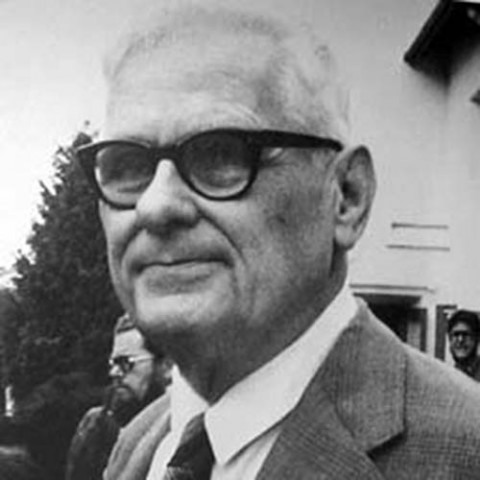
\includegraphics[width=\textwidth]{Church.jpeg}
        \column{0.5\textwidth}
        {\Large Alonzo Church} (1903 - 1995) 

        \emph{Princeton University, USA}
        \begin{itemize}
            \item<2-> Logicus, wiskundige
            \item<3-> Van 1936 tot 1979 redacteur van \emph{Journal of Symbolic Logic}
            \item<4-> 'Bedenker' van de $\lambda$-calculus
            \item<5-> Eerste-orde predicaat-logica is onbeslisbaar
            \item<6-> Peano-arithmetiek is onbeslisbaar
        \end{itemize}    
    \end{columns}
\end{frame}

\begin{frame}
    \frametitle{De protagonisten}
    \begin{columns}
        \column{0.5\textwidth}
        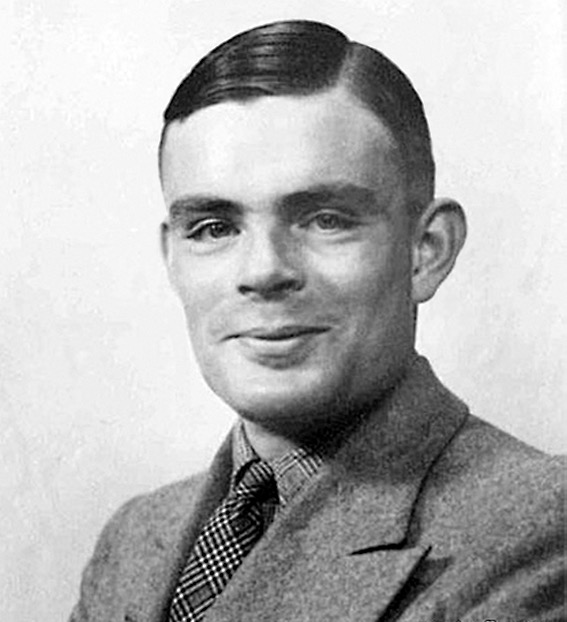
\includegraphics[width=\textwidth]{Turing.jpg}
        \column{0.5\textwidth}
        {\Large Alan Turing} (1912 - 1954) 

        \emph{Cambridge \& Manchester}
        \begin{itemize}
            \item Grondlegger van
            \begin{itemize}
                \item<2-> Informatica
                \item<3-> Artificiële intelligentie
                \item<4-> Morphogenetica
            \end{itemize}
            \item<5-> Legendarisch codebreaker
            \item<6-> Marathonloper
            \item<7-> Homosexueel in een tijd dat het strafbaar was
        \end{itemize}    
    \end{columns}
\end{frame}

\begin{frame}
    \frametitle{De protagonisten}
    \begin{tabular*}{\textwidth}{c c}
        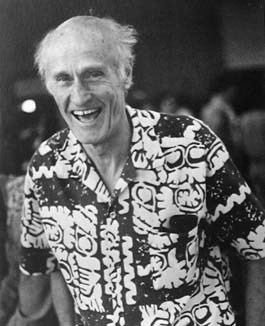
\includegraphics[width=0.4\textwidth]{Kleene.jpeg} & \includegraphics[width=0.4\textwidth]{example-image-duck} \\
        {\large Stephen Kleene} (1909-1994) & {\large ???} (1897 - 1954)\\
    \end{tabular*}
\end{frame}

\section{De situatie}
\subsection{Entscheidungsproblem}
\begin{frame}
    \frametitle{Das Entscheidungsproblem}
    {\large \textbf{Das Entscheidungsproblem}}

    \begin{center}
        Vind een algoritme waarmee \\ 
        de waarheid van een uitspraak in de eerste orde predikaatlogica \\
        vast te stellen is.
        \\
        \bigskip
        {\small \emph{(D. Hilbert \& W. Ackermann, 1928, Grundzüge der theoretischen Logik)}}
    \end{center}
\end{frame}

\begin{frame}
    \frametitle{Entscheidungsproblem}
    \textbf{Eerste orde predikaatlogica} \\
    (extreem kort door de bocht) 
    \bigskip
    
    Logica met
    \begin{itemize}
        \item<2-> variabelen
        \item<3-> de gebruikelijke operatoren $\wedge, \vee, \rightarrow, \neg, \ldots$
        \item<4-> predikaten $P(x)$
        \item<5-> universele en existentiële kwantificatie $\forall, \exists$
    \end{itemize}

    \onslide<6->{Voorbeelden:}
    \onslide<7->{$$\forall_{n \in \mathbb{N}}\exists_{m \in \mathbb{N}} [m>n]$$}
    \onslide<8->{$$\forall_{p, q \in \mathbb{Q}} \exists_{r \in \mathbb{Q}}  [ p < r < q]$$}
    \onslide<9->{$$\exists_x [P(x)\wedge \forall_y \forall_{y'}[P(y) \wedge P(y') \rightarrow y = y']]$$}
\end{frame}

\begin{frame}
    \frametitle{Entscheidungsproblem}
    \textbf{Eerste orde predikaatlogica} \\

    \emph{Afspraak:}

    We hebben het alleen over predikaten en kwantificatie over de natuurlijke getallen $\mathbb{N}$

    \vspace{1cm}

    \onslide<2->{\emph{Gezocht: }}
    
    \onslide<3->{\textbf{Algoritme}
    
    wat gegeven een uitspraak roept of die uitspraak \texttt{WAAR} of \texttt{ONWAAR} is.}

    \vspace{1cm}
    \onslide<4->{
    \emph{Probleem: }
    
    Wat is een algoritme?}
\end{frame}

\subsection{Berekenbaarheidsmodellen}
\begin{frame} 
    \frametitle{Wat is een algoritme}
    {\Large Wat is een algoritme??}
    
    Reeds informeel bekend in de wiskunde
    \vspace{1cm}
    \begin{itemize}
        \item<2-> Grootste-gemene-deler van Euclides
        \item<3-> Zeef van Eratosthenes
        \item<4-> Gauss-eliminatie
    \end{itemize}
\end{frame}
\begin{frame} 
    \frametitle{Wat is een algoritme}

    \textbf{Probleem:} Nog geen \emph{formele} definitie van een \emph{algoritme}.
    \\
    \vspace{1cm}
    \onslide<2->{Terug naar 1936\only<3->{-ish}.}
        \begin{itemize}
            \item<4-> Turing machines
            \item<5-> Recursietheorie
            \item<6-> $\lambda$-calculus
        \end{itemize}        
\end{frame}

\begin{frame}
    \frametitle{De $\lambda$-calculus (\emph{Church 1932})}
    \textbf{De programma's}
    \begin{align*}
        \onslide<2->{x,y,\ldots \in \Lambda & \text{  (Variabelen)}\\}
        \onslide<3->{M,N\in \Lambda \Rightarrow MN \in \Lambda & \text{  (Applicatie)} \\}
        \onslide<4->{x, M\in \Lambda \Rightarrow (\lambda x.M) \in \Lambda & \text{  (Abstractie)}}
    \end{align*}
    \begin{columns}
        \column{0.5\textwidth}
        \begin{itemize}
            \item<5-> $\lambda x.x$
            \item<6-> $\lambda xy.x$
            \item<7-> $\lambda pqr.pr(qr)$
        \end{itemize}
        \column{0.5\textwidth}
        \begin{itemize}
            \item<8-> $(\lambda x.xx)A$
            \item<9-> $\lambda x.y$
            \item<10-> $\lambda fx.f(f(f(x))) \equiv \ulcorner 3 \urcorner$
        \end{itemize}    
    \end{columns}
\end{frame}

\begin{frame}
    \frametitle{De $\lambda$-calculus (\emph{Church 1932})}

    \textbf{Actie}

    $$(\lambda x.M)N \longrightarrow_\beta M [x:=N]$$

    \onslide<2->{
            
        \textbf{Voorbeeld}
        
        \begin{align*}
            \onslide<3->{(\lambda xyz.zxy)(\mathcolor{red}{\lambda x.xx})(\mathcolor{blue}{\lambda x.x})(\lambda xy.x) & \rightarrow_\beta \\}
            \onslide<4->{(\lambda yz.z(\mathcolor{red}{\lambda x.xx})y)(\mathcolor{blue}{\lambda x.x})(\lambda xy.x) & \rightarrow_\beta \\}
            \onslide<5->{(\lambda z.z(\mathcolor{red}{\lambda x.xx}))\mathcolor{blue}{\lambda x.x}(\lambda xy.x) & \rightarrow_\beta \\}
            \onslide<6->{(\lambda xy.x)(\mathcolor{red}{\lambda x.xx}))\mathcolor{blue}{\lambda x.x} & \twoheadrightarrow_\beta  \mathcolor{red}{\lambda x.xx}\\}
        \end{align*}
    }
    \onslide<7->{Nu jij: $(\lambda xyz.zxy)(\text{"the force"})(\text{"is"})(\text{"strong in you"})$}
\end{frame}

\begin{frame}
    \frametitle{Recursietheorie (\emph{Kleene 1935})}
    \onslide<2->{\textbf{Initiële functies}}
    \begin{align*}
        \onslide<3->{\mathcal{O}(x) & = 0 & \text{Nul}\\}
        \onslide<4->{\mathcal{S}(x) & = x + 1 & \text{Successor}\\}
        \onslide<5->{\mathcal{P}^n_i(x_1, \ldots, x_n) & = x_i & \text{Projectie} \\}
        \onslide<6->{f(\vec{x}) & = h(g_1(\vec{x}), \ldots, g_m(\vec{x})) & \text{Functie compositie}}
    \end{align*}
    \onslide<7->{\textbf{Primitieve recursie}}
    \begin{align*}
        \onslide<8->{f(\vec{x},0)   & = g(\vec{x}) & \text{0-geval} \\}
        \onslide<9->{f(\vec{x},n+1) & = h(\vec{x}, y, f(\vec{x},y)) & \text{Recursieve geval}}
    \end{align*}
    \onslide<10->{\textbf{$\mu$-recursie}}
    \begin{align*}
        \onslide<11->{f(\vec{x}) & = \mu y[g(\vec{x},y)=0] \\
           & \text{"De kleinste $y$ zodat $g(\vec{x},y)=0$"}}
    \end{align*}
\end{frame}

\begin{frame}
    \frametitle{Recursietheorie (\emph{Kleene 1935})}
    \textbf{Voorbeelden}
    \begin{columns}
        \onslide<2->{\column{0.5\textwidth}
            \begin{align*}
                \mathcal{P} (0) & = 0 \\
                \mathcal{P} (n + 1) & = n
            \end{align*}}
        \onslide<3->{\column{0.5\textwidth}
            \begin{align*}
                \min (x,0) & = x \\
                \min (x, y+1) & = \mathcal{P}(\min (x,y))
            \end{align*}}
        \end{columns}
        \vspace{1cm}
        \onslide<4->{$$f(n) = \mu y [2y= n \vee 2y+1 = n]$$}
\end{frame}

\begin{frame}
    \frametitle{Turing machines (\emph{Turing 1936})}
    \begin{columns}
        \column{0.5\textwidth}
            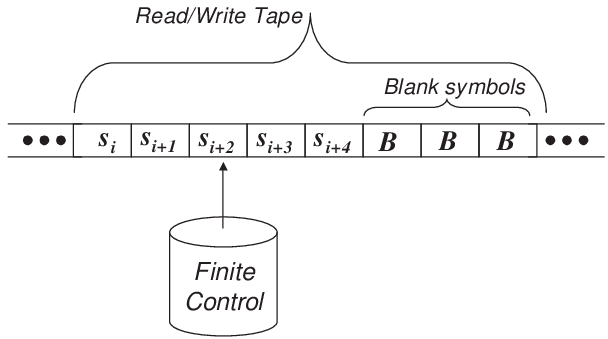
\includegraphics[width=0.8\textwidth]{tm.png}
        \column{0.5\textwidth}
            \begin{itemize}
                \item<2-> Een eindig alfabet $s_0, s_1, \ldots, s_n$
                \item<3-> Een eindig aantal toestanden $q_0, q_1, \ldots, q_m$
                \item<4-> Een potentieel oneindige tape voor de symbolen
                \item<5-> De acties: $L, R, s_i$.
                \item<6-> Een eindige lijst van instructies
            \end{itemize}
    \end{columns}
\end{frame}

\begin{frame}{}
    \frametitle{Turing machines (\emph{Turing 1936})}
    \begin{center}
        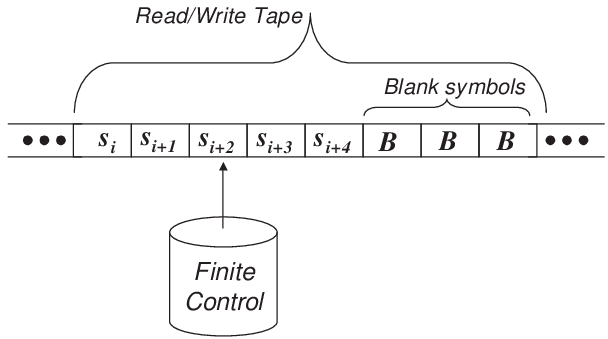
\includegraphics[height=0.3\textheight]{tm.png}
    \end{center}    
    \textbf{Voorbeeldinstructies}
    \begin{description}
        \item<2->[$q_0\mathbf{0}Rq_1$] Wanneer er in toestand $q_0$ een $\mathbf{0}$ op 
        de tape staat, zet een stap naar rechts en ga in toestand $q_1$.
        \item<3->[$q_4\mathbf{1}\mathbf{0}q_8$] Wanneer er in toestand $q_4$ een $\mathbf{1}$
        op de tape staat, vervang de $\mathbf{0}$ door een $\mathbf{1}$ en ga in toestand $q_8$.
    \end{description}
\end{frame}

\begin{frame}
    \frametitle{De equivalentie}

    $$\lambda-\text{definieerbaar} \stackrel{\scriptscriptstyle \text{(Turing 1937)}}{\Longrightarrow} \text{Turing berekenbaar}$$

    \onslide<2->{$$\text{Turing berekenbaar} \stackrel{\scriptscriptstyle \text{(Turing 1937)}}{\Longrightarrow} \mu-\text{recursief} $$}

    \onslide<3->{$$\mu-\text{recursief} \stackrel{\scriptscriptstyle \text{(Kleene 1936)}}{\Longrightarrow} \lambda-\text{definieerbaar} $$}
\end{frame}

\begin{frame}
    \frametitle{De equivalentie}

    De uitspraken:
    \begin{itemize}
        \item<2-> Een functie $f:\mathbb{N} \rightarrow \mathbb{N}$ is berekenbaar
        \item<3-> Er bestaat een $\lambda$-term $F$ zdd $f(n) = m \Leftrightarrow F \ulcorner n\urcorner = \ulcorner m\urcorner $
        \item<4-> Er bestaat een $\mu$-recursieve functie $\phi$ zdd $f(n) = m \Leftrightarrow \phi(n) = m$
        \item<5-> Er bestaat een T.M. zdd $f(n) = m \Leftrightarrow \text{T.M.}_f \text{ geeft bij invoer } \ulcorner n\urcorner \text{ uitvoer } \ulcorner m\urcorner$
    \end{itemize}
    \vspace{0.5cm}
    \onslide<6->{zijn synoniem met elkaar.}
\end{frame}

\subsection{De kracht van berekenbaarheid}
\begin{frame}
    \frametitle{Halting Problem}
    {\Large Iets met oneindigheid}
    \vspace{1cm}

    \textbf{Probleem:}

    Een algoritme kan eindeloos lang doorgaan, zonder een 'antwoord' te geven.\\
    \vspace{1cm}

    \begin{tabular*}{0.8\textwidth}{r l}
        \onslide<2->{$\lambda$-calculus & $(\lambda x.xx)(\lambda x.xx)$ \\}
        \onslide<3->{Recursietheorie & $f(n) = \mu y [y<0]$ \\}
        \onslide<4->{Turing machine & $\{ q_0\mathbf{0}\mathbf{0}q_1, q_1\mathbf{0}\mathbf{0}q_0 \}$}
    \end{tabular*}
\end{frame}

\begin{frame}
    \frametitle{Halting Problem}
    {\Large Iets met oneindigheid}
    \vspace{1cm}

    \textbf{Probleem:}

    Een algoritme kan eindeloos lang doorgaan, zonder een 'antwoord' te geven.\\
    \vspace{1cm}

    \onslide<2->{\textbf{Oplossing:}

    Schrijf een algoritme wat van een gegeven algoritme $P$ bepaalt of deze bij gegeven invoer $n$ een antwoord geeft.}

    \begin{center}
    \only<3->{\Large \color{red}\textbf{Computer says no...}}
    \end{center}
\end{frame}

\begin{frame}
    \frametitle{Halting Problem}

    \begin{theorem}[Halting Problem]
        Er bestaat geen algoritme wat bepaalt of een gegeven algoritme $P$ stopt bij gegeven invoer $n$.
    \end{theorem}
    \onslide<2->{
    \begin{proof}
        Stel dat er een algoritme $H$ bestaat (*), wat aan de voorwaarden voldoet.}
        \onslide<3->{Maak een nieuw algoritme $H'$ op de volgende manier:
        \[
            H'(n) = \begin{cases}
                \uparrow & \text{als $H(P,n)=1$} \\
                1 & \text{als $H(P,n)\uparrow$}
            \end{cases}
        \]}
        \onslide<4->{
        Beschouw nu $H(H'(n))$. Wanneer $H$ oneindig draait, is $H'$ gedefinieerd, maar dan 
        zou $H$ juist niet oneindig moeten draaien. Tegenspraak.} 
        \onslide<5->{We geven de aanname (*) de schuld.}
    \end{proof}
\end{frame}

\begin{frame}{}
    \frametitle{Entscheidungsproblem}

    \onslide<1->{\textbf{Feit:} Er zijn overaftelbaar veel onoplosbare problemen}
    
    \vspace{1cm}
    
    \onslide<2->{\textbf{Nog zo een:} Het is \emph{niet} beslisbaar om van een 
    gegeven programma $P$ te zeggen of het uitvoer $x$ geeft.}
    
    \vspace{1cm}
    
    \onslide<3->{\textbf{Gevolg:} Het \emph{Entscheidungsproblem} is niet oplosbaar.}
\end{frame}

\begin{frame}
    \frametitle{Universaliteits principe}
    $$\text{Beslisbaar probleem $P$} \Longrightarrow 
      \text{T.M voor probleem $P$}$$

    \vspace{1cm}
    \onslide<2->{\textbf{The ugly:}Erg veel T.M.'s}
 
    \onslide<3->{\textbf{Gezocht:}}
    \vspace{0.5cm}
    \onslide<4->{\begin{center}
        \textbf{One TM to rule them all}
    \end{center}}
\end{frame}

\begin{frame}
    \frametitle{Universaliteits principe}
    \begin{center}
        \textbf{One TM to rule them all}
    \end{center}

    \textbf{Hoe?}
    \onslide<2->{\begin{proof}
        Bereken een \emph{beschrijvend getal} $e$ per T.M $M$
        
        (een soort Gödelcodering van T.M.'s)}

        \onslide<3->{Maak een T.M. $U$, die een programma $e$ en een invoer vraagt.}

        \onslide<4->{Nu geeft $U(e,n)$ het antwoord $p$ op de tape precies wanneer $M$ antwoord $p$ geeft bij invoer $n$.}
    \end{proof}

    \onslide<5->{Machine $U$ noemen we een \emph{Universele Turingmachine}.}
    
    \onslide<6->{In effect een \emph{Interpreter}.}
\end{frame}

\begin{frame}{}
    \frametitle{Tussentijdse terugblik}
    {\Large Terugblik}
    \begin{itemize}
        \item<2-> Formele definitie van een algoritme
        \item<3-> \emph{Berekenbaarheid}
        \item<4-> Best veel onberekenbare problemen
        \item<5-> Reële getallen op een computer, foggeddaboudid.
        \item<6-> De droom van Hilbert in scherven
        \item<7-> One machine to rule them all
    \end{itemize}
    \onslide<8->{
    \begin{center}
        {\textbf{Op naar de These!}
        }
    \end{center}
    }
\end{frame}

\section{De these}
\begin{frame}
    \frametitle{De These}
    \begin{center}
        {\Large
            Every \emph{effectively calculable} function is \emph{computable}
        }
        \\
        Church (1936), Turing (1937)

        Elke \emph{uitrekenbare} functie is \emph{berekenbaar}
    \end{center}
\end{frame}


\section{Voorbij de these}
\subsection{Echte computers}
\begin{frame}{}
    \frametitle{Concrete Turing Machines}
    \begin{itemize}
        \item<2-> Colossus (1943)
        \item<3-> ENIAC (1946)
        \item<4-> Automatic Computing Engine (1945)
        \item<5-> EDVAC, EDSAC (1949)
    \end{itemize}

    \onslide<6->{Belangrijk concept: \emph{Stored Program Computer} (von Neumann, 1945)}
\end{frame}

\subsection{Hypercomputation}
\begin{frame}{}
    \frametitle{To boldly go where no man has gone before}

    \begin{itemize}
        \item<2-> Orakel machines (Turing, 1939)
        \item<3-> Infinite state machines (discussie Gödel)
        \item<4-> Black hole
        \item<5-> Quantum computing 
    \end{itemize}
\end{frame}

\subsection{Quantum computing}
\begin{frame}
    \frametitle{Quantum computing}

    \begin{itemize}
        \item<2-> Superpositie
        \item<3-> Interferentie
        \item<4-> Verstrengeling
    \end{itemize}

    \vspace{0.5cm}
    \onslide<5->{\textbf{Gevolgen voor:}}
    \begin{itemize}
        \item<6-> Cryptografie
        \item<7-> Zoek algoritmen
        \item<8-> Computationele biologie
        \item<9-> Machine learning?
    \end{itemize}
\end{frame}

\begin{frame}{}
    \frametitle{Quantum computing}
    \begin{block}{Church-Turing-Deutsch These}
        Een universele computer kan elk fysisch proces simuleren
        
        {\small Gandy 1980, Deutsch 1985}
    \end{block}

    \onslide<2->{
    \begin{block}{Stelling}
        De klasse van \emph{berekenbare functies} \\
        is \emph{gelijk} aan \\
        de klasse van \emph{quantum-berekenbare} functies.
    \end{block}
    }
\end{frame}

\begin{frame}{}
    \frametitle{Terugblik}
    \begin{itemize}
        \item<2-> Kennis over algoritmen en berekenbaarheid
        \item<3-> Van abstracte logica naar je broekzak
        \item<4-> Harde grenzen
        \item<5-> \emph{Mer à boire}
        \item<6-> ?? 
    \end{itemize}
\end{frame}

\begin{frame}{}
    \frametitle{The End}

    {\LARGE Dankjewel voor je aandacht}
    
    \vspace{3cm}

    Contact: mail@pietervanengelen.nl
\end{frame}

%\section*{Tragiek in het paradijs}
\begin{frame}
    \begin{center}
        {\LARGE Tragiek in het paradijs}
    \end{center}
\end{frame}

\begin{frame}
    \frametitle{De protagonisten}
    \begin{tabular*}{\textwidth}{c c}
        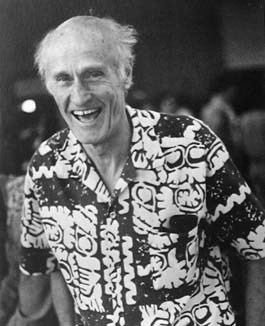
\includegraphics[width=0.4\textwidth]{Kleene.jpeg} & \includegraphics[width=0.4\textwidth]{example-image-duck} \\
        {\large Stephen Kleene} (1909-1994) & {\large ???} (1897 - 1954)\\
    \end{tabular*}
\end{frame}

\begin{frame}
    \frametitle{De protagonisten}
    \begin{tabular*}{\textwidth}{c c}
        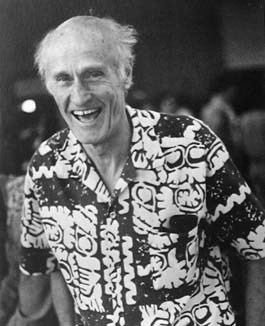
\includegraphics[width=0.4\textwidth]{Kleene.jpeg} & 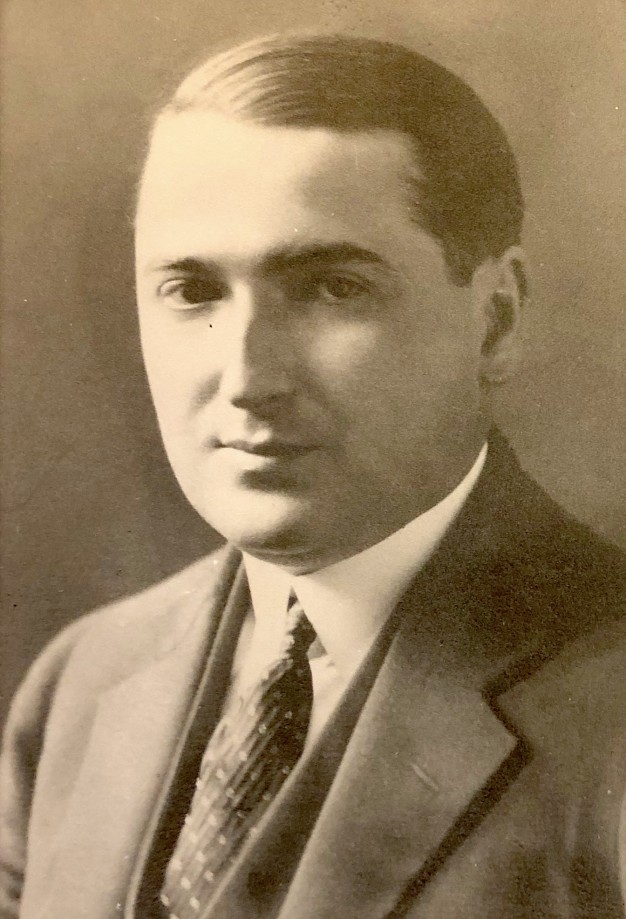
\includegraphics[width=0.4\textwidth]{Post.jpg} \\
        {\large Stephen Kleene} (1909-1994) & {\large Emil Post} (1897 - 1954)\\
    \end{tabular*}
\end{frame}

\begin{frame}{}
    \frametitle{Emil Leon Post}
    \begin{columns}
        \column{0.4\textwidth}
        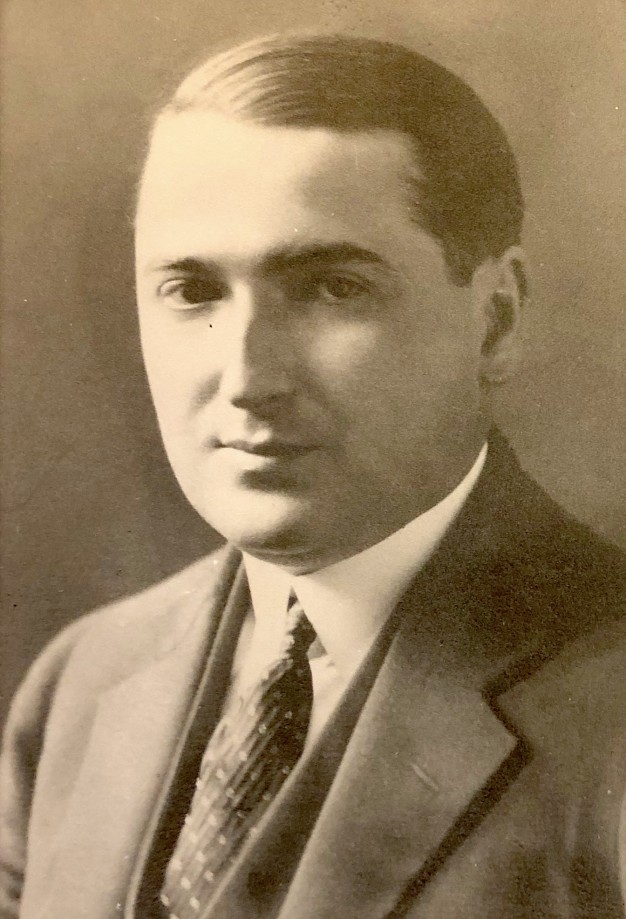
\includegraphics[height=0.8\textheight]{Post.jpg}
        \column{0.6\textwidth}
        {\small
        \begin{itemize}
            \item<2-> Logicus en wiskundige
            \item<3-> Bewijs van volledigheid propositielogica uit \emph{Principia Mathematica} (1919) 
            \item<4-> Vond in 1920 aanwijzingen voor de Onvolledigheidsstellingen van Gödel 
            en onbeslisbaarheidsresultaten van Church en Turing
            \item<5-> Bipolaire stoornis
            \item<6-> Finite Combinatory Processes (1936)
            \item<7-> Turing-degree/Post's Theorem (1944)
        \end{itemize}
        }
    \end{columns}        
\end{frame}

\end{document}